\documentclass[12pt]{beamer}
\usepackage[english, russian]{babel}
\usepackage[utf8x]{inputenc}
\usepackage{itmobeamer}
\usepackage{makecell}
\usepackage{tabularx}
\usepackage{multicol}
\usepackage{caption}
\usepackage{listings}
\usepackage{subcaption}

\lstset{emph={
    tc, qdisc, class, dev, parent, classid, filter, protocol, flowid, cbwfq, default, bandwidth,
    },emphstyle={\bfseries}%
}%


\title[Исследование и реаализация ДО CBWFQ]{Исследование и реализация взвешенного алгоритма честного обслуживания на основе классов\\}
\author[]{{\small Автор: Куклина Мария Дмитриевна\\ Научный руководитель: Шинкарук Дмитрий Николаевич}}
\institute[]{Университет ИТМО}
\date[]{Санкт-Петербург, 2018}

\begin{document}

\newcommand{\mc}[0]{\makecell}
\newcommand\setrow[1]{\gdef\rowmac{#1}#1\ignorespaces}
\newcommand\clearrow{\global\let\rowmac\relax}
\clearrow
%\itmologoslide

\begin{darkbars}
    \begin{frame}[noheader,nologo,noframenumbering]
        \titlepage
    \end{frame}
\end{darkbars}

\begin{frame}{Цели и задачи}
    \textbf{Цель} -- реализация дисциплины обслуживания Class-Based Weighted Fair Queueing
    (CBWFQ) в ядре Linux. \newline
    

    \textbf{Задачи}
    {\small
        \begin{itemize}
            \item Провести сравнительный анализ CBWFQ с рядом выбранных дисциплин обслуживания.
            \item Настроить среду для реализации и тестирования.
            \item Реализовать CBWFQ в ядре Linux.
            \item Добавить интерфейс в утилиту tc для работы с ДО.
        \end{itemize}
    }
\end{frame}

%\begin{frame}{Качество обслуживания}
%
%	%\textbf{Качество обслуживания (QoS)} -- технология предоставления разным классам трафика различное обслуживание.
%
%	\textbf{Пропускная способность (bandwidth, ПС)} -- характеристика канала, описывающая объем данных, который может быть передан через канал.
%
%	\textbf{Задержка (latency)} -- задержка передачи пакета в сети.
%
%	\textbf{Простой (starvation)} -- отсутствие обслуживания в длительное время.
%	
%	\textbf{Разделение канала (link sharing)} -- механизм разделения канала между потоками трафика,
%	при котором канал, который не занят одним типом трафика, одалживается другому типу трафика.
%
%	\textbf{Честность (fairness)} -- мера честного распределения ресурсов; в общем случае обозначает
%	равенство распределение ресурсов.
%
%\end{frame}

\begin{frame}{Дисциплины обслуживания}
	% TODO: сделать рисунок более понятным
	\textbf{Дисциплина обслуживания (qdisc, ДО)} -- набор алгоритмов,
	определяющий метод организации очереди, способы выбора пакета из очереди,
	политику отбрасывания пакетов и способы выделения канала.
	\begin{figure}
		\center
    	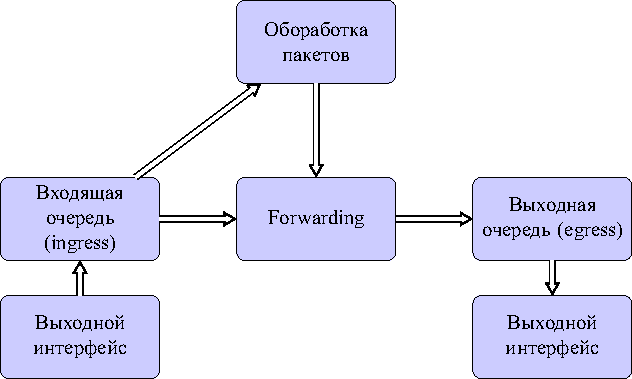
\includegraphics[scale=0.7]{../text/src/pdfimages/qdisc.pdf}
	\end{figure}


\end{frame}

\begin{frame}{Priority Queueing}
	\begin{figure}
		\center
    	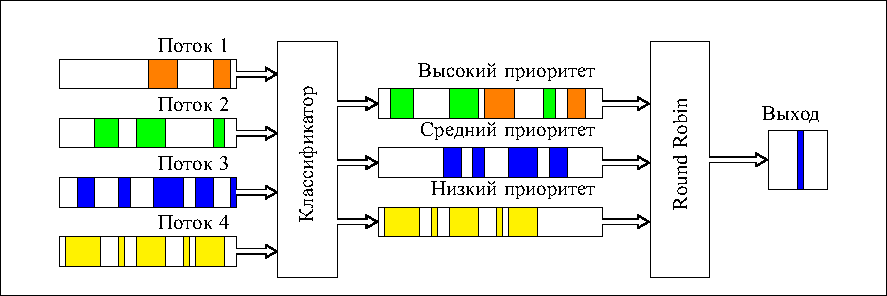
\includegraphics[scale=0.6]{../text/src/pdfimages/pq.pdf}
	\end{figure}
	\begin{center}
        {\footnotesize
            \begin{multicols}{2}
				{\bf Преимущества}
				\begin{itemize}
					\item Низкое время отклика.
					\item Простая реализация.
					\item Небольшая вычислительная нагрузка.
				\end{itemize}
            \columnbreak
				{\bf Недостатки}
				\begin{itemize}
					\item Проблема простоя канала.
					\item Избыточный трафик увеличивает задержку.
					\item Простой низкоприоритетного трафика при избытке высокоприоритетного.
				\end{itemize}
            \end{multicols}
        }
	\end{center}
\end{frame}

\begin{frame}{Class Based Queueing}
	\begin{figure}
		\center
    	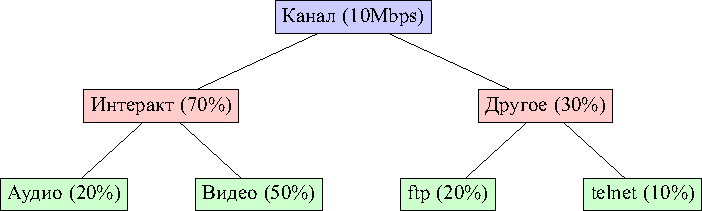
\includegraphics[scale=0.6]{../text/src/pdfimages/cbq.pdf}
	\end{figure}


	\begin{center}
        {\footnotesize
            \begin{multicols}{2}
				{\bf Преимущества}
				\begin{itemize}
					\item Разделение канала.						  
					\item Решение проблемы застоя канала.
				\end{itemize}
            \columnbreak
				{\bf Недостатки}
				\begin{itemize}
					\item Честное выделение канала только для пакетов сравнительно одинакового размера.
					\item Слабо оптимизирована для большинства типичных ситуаций.
					\item Сложность реализации.
				\end{itemize}
            \end{multicols}
        }
	\end{center}
\end{frame}

\begin{frame}{Hierarchy Token Bucket}
%	\begin{figure}
%		\center
%    	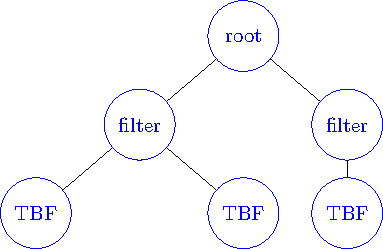
\includegraphics[scale=0.7]{../text/src/pdfimages/class_hierh_htb.pdf}
%	\end{figure}
\begin{figure}
  \begin{subfigure}[b]{0.35\textwidth}
   	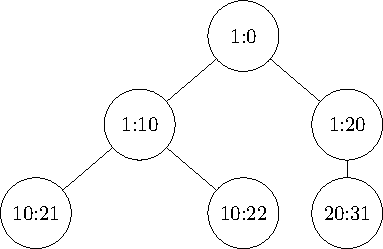
\includegraphics[width=\textwidth]{../text/src/pdfimages/class_hierh.pdf}
    \label{fig:f1}
  \end{subfigure}
  \hspace{0.2\textwidth}
  \begin{subfigure}[b]{0.35\textwidth}
   	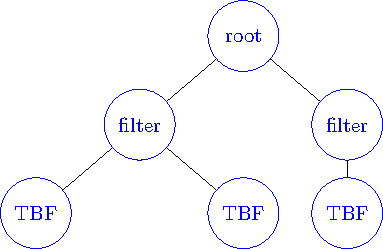
\includegraphics[width=\textwidth]{../text/src/pdfimages/class_hierh_htb.pdf}
    \label{fig:f2}
  \end{subfigure}
\end{figure}
	\begin{center}
    {\footnotesize
            \begin{multicols}{2}
				{\bf Преимущества}
				\begin{itemize}
					\item Гикая конфигурация.
					\item Разделение канала.
					\item Более простая реализация, чем у CBQ.
					\item Используется для ограничения клиентской скорости.
				\end{itemize}
            \columnbreak
				{\bf Недостатки}
				\begin{itemize}
					\item Честное выделение канала только для пакетов сравнительно одинакового размера.
					\item Сложность реализации.
				\end{itemize}
            \end{multicols}
    }
	\end{center}
\end{frame}

\begin{frame}{HFSC}

\begin{figure}
  \begin{subfigure}[b]{0.3\textwidth}
     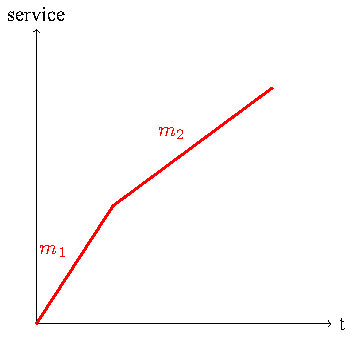
\includegraphics[width=\textwidth]{../text/src/pdfimages/hfsc_concave.pdf}
    \caption*{{\scriptsize Вогнутая (concave) кривая.}}
    \label{fig:f1}
  \end{subfigure}
  \hspace{0.2\textwidth}
  \begin{subfigure}[b]{0.3\textwidth}
    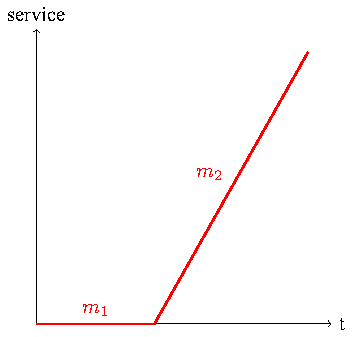
\includegraphics[width=\textwidth]{../text/src/pdfimages/hfsc_convex.pdf}
    \caption*{{\scriptsize Выпуклая (convex) кривая.}}
    \label{fig:f2}
  \end{subfigure}
\end{figure}


	\begin{center}
    {\footnotesize
            \begin{multicols}{2}
				{\bf Преимущества}
				\begin{itemize}
					\item Основан на формальной модели с доказанными нижними границами.
				\end{itemize}
            \columnbreak
				{\bf Недостатки}
				\begin{itemize}
					\item Высокая сложность реализации.
				\end{itemize}
            \end{multicols}
        }
	\end{center}
\end{frame}

\begin{frame}{Weighted Fair Queueing}
	

	\textbf{General Processor Sharing (GPS)} -- математическая модель
	планировщика, позволяющая максимально точно разделить пропускную
	способность между классами трафика в соответствии с назначенными
	весами.

	\textbf{WFQ} -- взвешенный алгоритм честного обслуживания,
	представляющий собой аппрокисмацию модели GPS; он оперирует
	пакетами, предоставляя максимально честное обслуживание,
	которое возвомжно для данного алгоритма при работе с пакетами.

\end{frame}

\begin{frame}{WFQ Drop Policy}
	\begin{figure}
		\center
    	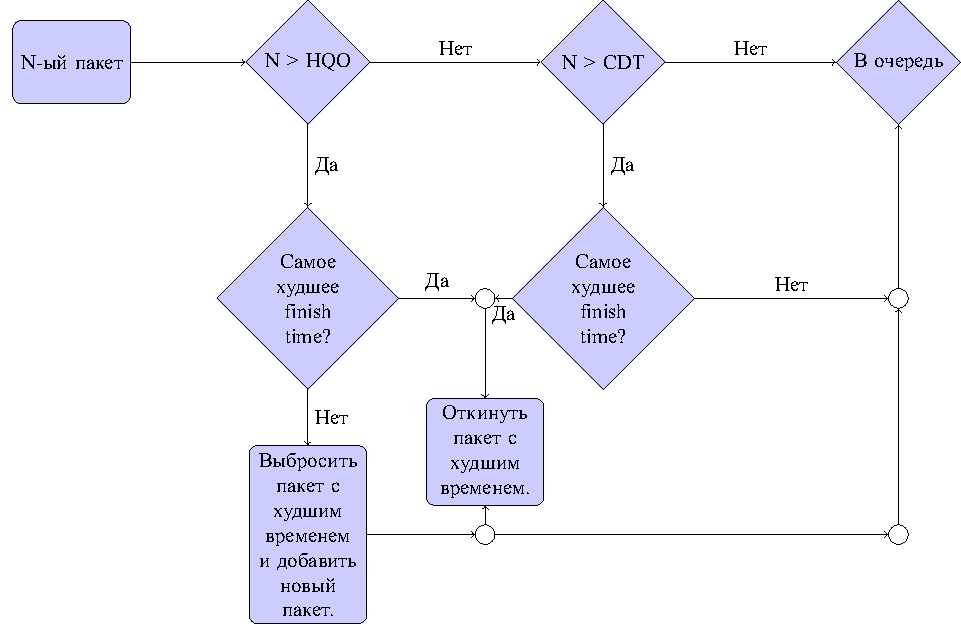
\includegraphics[scale=0.6]{../text/src/pdfimages/fwfq_drop.pdf}
	\end{figure}
	%{\scriptsize
	%CDT (congestive discard threshold) -- количество пакетов в системе WFQ перед началом отбрасывания.\\
	%HQO (hold queue out) -- максимальное количество пакетов во всех выходящих очередях.
	%}
\end{frame}

\begin{frame}{Flow-based Weighted Fair Queueing}
	\begin{figure}
		\center
    	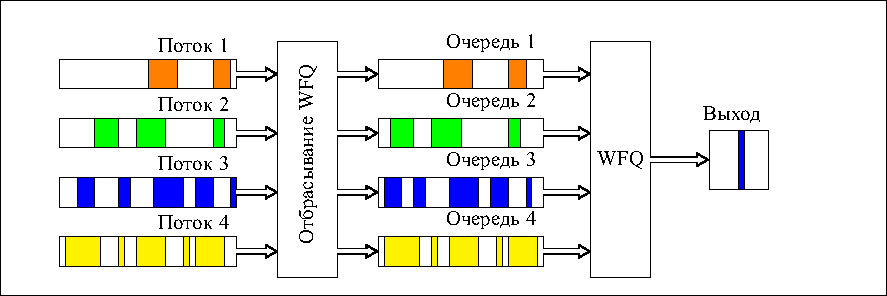
\includegraphics[scale=0.6]{../text/src/pdfimages/fwfq.pdf}
	\end{figure}
	\begin{center}
        {\footnotesize
            \begin{multicols}{2}
				{\bf Преимущества}
				\begin{itemize}
					\item Простая конфигурация.
					\item Гарантированная полоса пропускания для всех потоков.
					\item Отбрасывание пакетов из агрессивных потоков.
					\item Честное обслуживание.
				\end{itemize}
            \columnbreak
				{\bf Недостатки}
				\begin{itemize}
					\item Нельзя разделять трафик по классам обслуживания.
					\item Не предоставляет фиксированную пропускную способность.
				\end{itemize}
            \end{multicols}
		}
	\end{center}
\end{frame}

\begin{frame}{Class-Based Weighted Fair Queueing}
	\begin{figure}
		\center
    	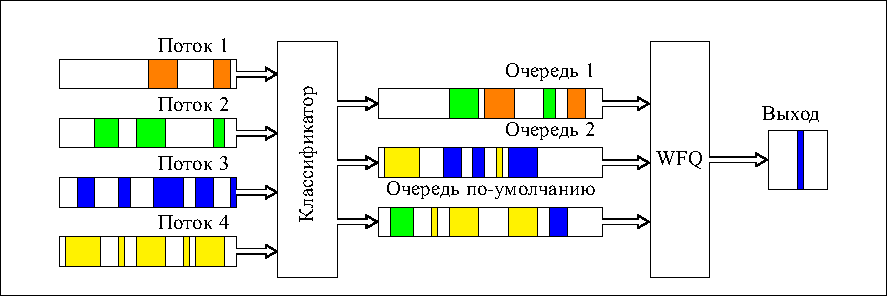
\includegraphics[scale=0.7]{../text/src/pdfimages/cbwfq.pdf}
	\end{figure}

	\begin{center}
{\footnotesize
            \begin{multicols}{2}
				{\bf Преимущества}
				\begin{itemize}
					\item Гибкая конфигурация классов.
					\item Выделение заданной пропускной способности для классов.
				\end{itemize}
            \columnbreak
				{\bf Недостатки}
				\begin{itemize}
					\item Ограничение на количество пользовательских классов.
					\item Плохо работает с интерактивным трафиком.
				\end{itemize}
            \end{multicols}
}
	\end{center}
\end{frame}

\begin{frame}{Сравнительная таблица ДО}
{\footnotesize
    \begin{tabular}{|>{\rowmac}c|>{\rowmac}c|>{\rowmac}c|>{\rowmac}c|>{\rowmac}c|>{\rowmac}c|>{\rowmac}c<{\clearrow}|}
        \hline
\setrow{\bfseries}               Свойство     & PQ   & CBQ   & HTB   & HFSC  & FWFQ  & CBWFQ \\ \hline
{\bf \mc{Метод\\ планирования}   }& RR   &WRR    & RR    & RT/LS & WFQ   & WFQ   \\ \hline
{\bf Честность                   }& -    & -     & -     & +     &  +    &  +    \\ \hline
{\bf      Отбрасывание           }&{\scriptsize  TD   }&{\scriptsize  TD    }&{\scriptsize  TD    }&{\scriptsize  TD    }&{\scriptsize  ED/AD }&{\scriptsize  TD/WRED }\\ \hline
{\bf \mc{Разделение\\ канала}    }& -    &  +    &  +    &  +    &  -    &  -    \\ \hline
{\bf \mc{Сложность \\ реализации}}& {\scriptsize Низкая }& {\scriptsize Высокая     }&  {\scriptsize Средняя    }&  {\scriptsize Высокая    }&   {\scriptsize Средняя   }&  {\scriptsize Средняя}\\ \hline
    \end{tabular}
}

{\scriptsize
	Обозначения:\\
	 RR -- Round Robin, RT/LS -- на основе Real Time/Link Sharing критериев.\\
	 TD -- Tail Drop, ED -- Early Dropping, ED -- Aggressive Dropping.
}
\end{frame}

%\begin{frame}{Исследование модели в Anylogic}
%	\begin{figure}
%		\center
%    	\includegraphics[scale=0.3]{./wfq_anylogic.png}
%		\caption{Среднее время ожидания пакета в системе при $W_1 = 0.7, W_2 = 0.3$}
%	\end{figure}
%
%	{\footnotesize W -- среднее время ожидания пакета в системе, мс.}
%\end{frame}

\begin{frame}[fragile]{Тестирование модуля}
	\begin{figure}
		\center
    	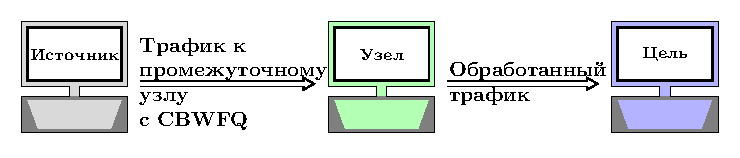
\includegraphics[scale=0.7]{../text/src/pdfimages/test_scheme.pdf}
		\caption*{{\footnotesize Схема тестовой среды}}
	\end{figure}
{\footnotesize
	\begin{lstlisting}[frame=single]
tc qdisc add dev eth1 cbwfq default limit 200
tc class add dev eth1 parent 1: classid 1:2\
 cbwfq bandwidth 30 percent  
tc class add dev eth1 parent 1: classid 1:3\
 cbwfq bandwidth 60 percent  
tc filter add dev ens3 parent 1: protocol ip\
 u32 match ip sport $TESTPORT1 flowid 1:2
tc filter add dev ens3 parent 1: protocol ip\
 u32 match ip sport $TESTPORT2 flowid 1:3
    \end{lstlisting}
}
\end{frame}

\begin{frame}{Тестирование модуля}
	\begin{figure}
		\center
    	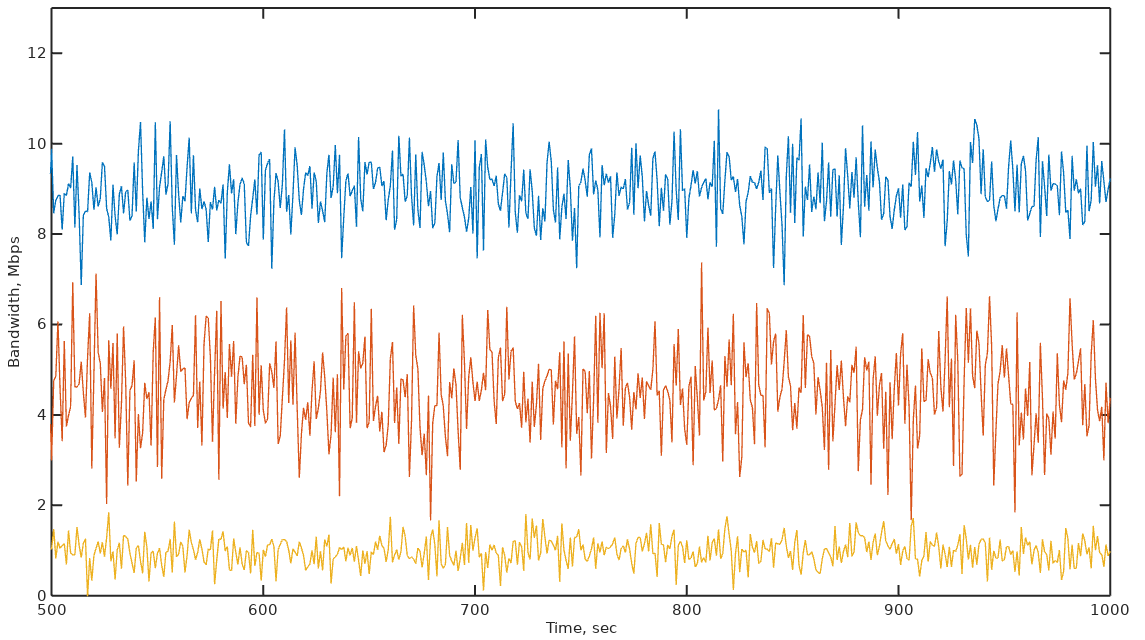
\includegraphics[scale=0.25]{./plot.png}
		\caption*{{\footnotesize График распределения пропускной способности по типам трафика в течение времени.}}
	\end{figure}
\end{frame}

\begin{frame}{Вывод}
	\begin{itemize}
		\item Проведён сравнительный анализ классовых дисциплин обслуживания.
		\item Проведено исследование модели WFQ в среде Anylogic.
		\item Реализован интерфейс для системы tc.
		\item Реализован алгоритм CBWFQ в ядре Linux.
	\end{itemize}
\end{frame}

\itmothankyou

\end{document}

